\documentclass{beamer} % Gliederung im Kopf, sections und subsections
\setbeamertemplate{navigation symbols}{}%remove navigation symbols

\usepackage{tikz}
\usetikzlibrary{shapes,arrows,positioning,chains,fit,calc,matrix,decorations.pathreplacing}
\usepackage{xcolor}
\usetikzlibrary{intersections}


\usepackage{tikz}
\usetikzlibrary{arrows,decorations.pathmorphing,backgrounds,positioning,fit,petri}
\renewcommand*{\familydefault}{\sfdefault}

\tikzset{forestyle/.style = {rectangle, thick, minimum width = 5cm, minimum height = 0.5cm, text width = 4.5cm, outer sep = 1mm},  
  pre/.style={<-, shorten <=1pt, >=stealth, ultra thick},
  extend/.style={<-,dashed, shorten <=1pt, >=stealth, ultra thick}}
  


\def\firstcircle{[name path=firstcircle] (0,0) circle (3cm)}
\def\secondcircle{[name path=secondcircle] (55:3.11111cm) circle (3cm)} %No idea how the numbers selected work; they were derived from what I found online. They seem to function though!
\def\thirdcircle{[name path=thirdcircle] (0:3.5cm) circle (3cm)}


\mode<presentation>

\begin{document}

\begin{frame}\begin{center}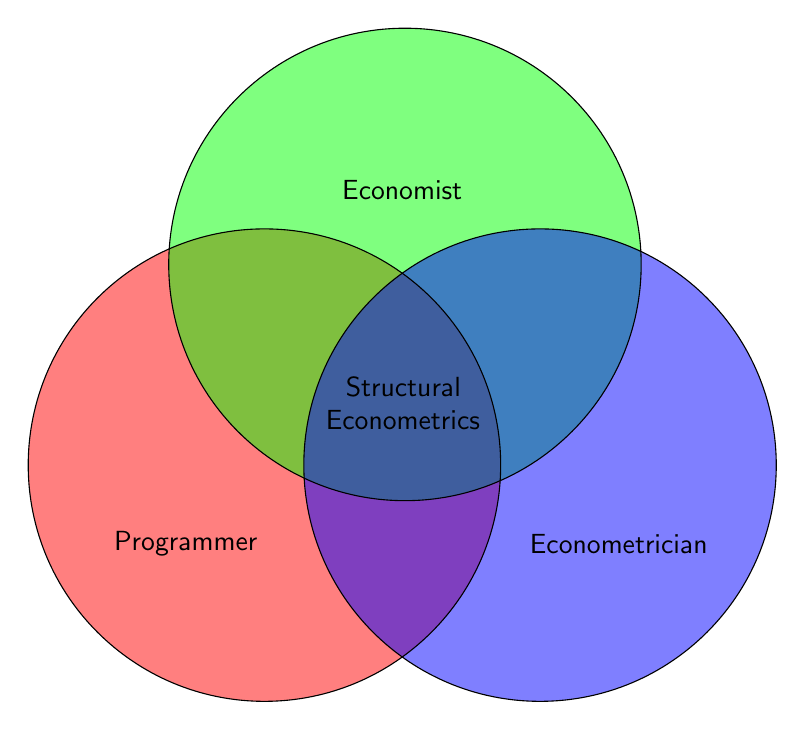
\begin{tikzpicture}
    \begin{scope}[fill opacity=.5, text opacity=1]
    \fill[red] \firstcircle;  
    \fill[green]\secondcircle;
    \fill[blue]\thirdcircle;
    \draw \firstcircle node[below,name=A] {};
    \draw \secondcircle node [above,name=B] {};
    \draw \thirdcircle node [below,name=C] {};
    \node at ($0.4*(B)+0.3*(C)+0.3*(A)$) {Structural}; 
    \node at ($0.25*(B)+0.375*(C)+0.375*(A)$) {Econometrics};
    \path (-1cm,-1cm) node {Programmer}
    (1.75cm,3.5cm) node {Economist}
    (4.5cm,-1cm) node {Econometrician};
    \end{scope}
\end{tikzpicture}\end{center}\end{frame}


\end{document}
